\chapter{Versuch 6: Aktiver Tiefpass erster Ordnung}

\section{Vorbereitung}

\subsection{Benötigte Geräte}

\begin{tabular}[h]{c|c}
    Widerstand 1 k$\Omega$ & 2\\
    \hline
    Widerstand 10 k$\Omega$ & 1\\
    \hline
    Operationsverstärker & \\
    \hline
    Netzgerät & Tenma 72-10495 Digital Control DC Power Supply\\
    \hline
    Funktionsgenerator & T3AFG80\\
    \hline
    Oszilloskop & Keysight DSOX1102A
    \label{tab:Versuch 6: Geräte}
\end{tabular}
\subsection{Schaltungsskizze}

\begin{figure}[H]
    \centering
    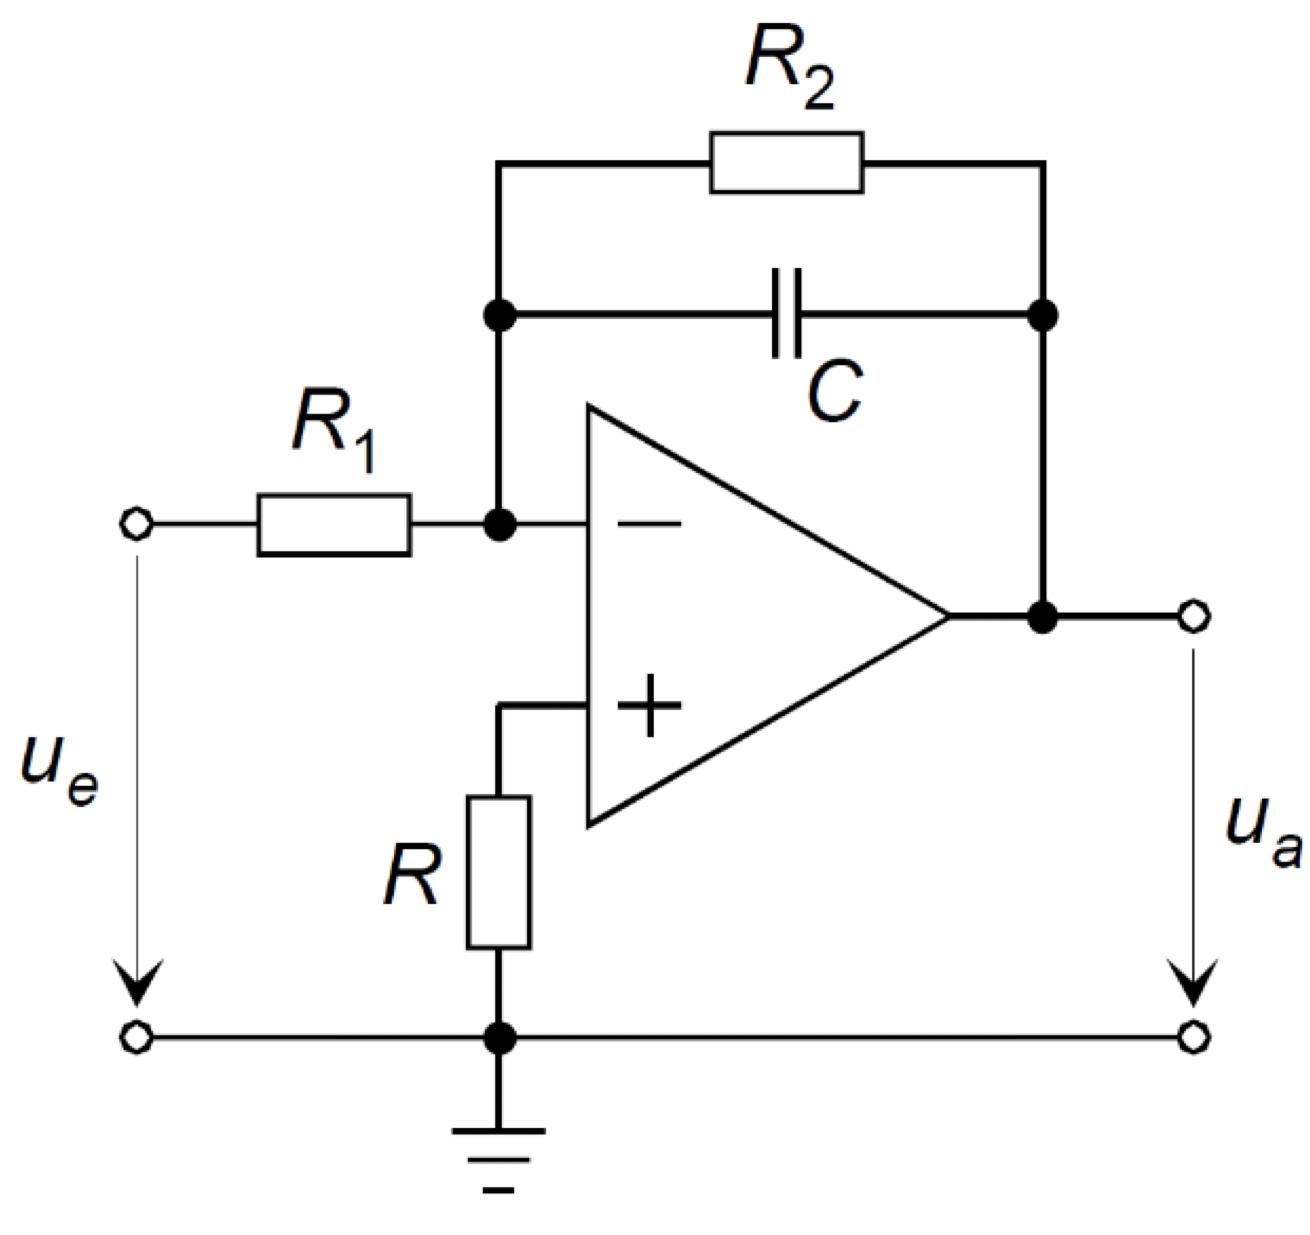
\includegraphics[height=7cm]{images/Versuch6/Schaltungsskizze.jpeg} 
    \caption{Schaltungsskizze}
    \label{fig: Schaltungsskizze}
\end{figure}
Gegebene Größen sind R\textsubscript{1} = 1k$\Omega$,
R\textsubscript{2} = 10k$\Omega$ und C = 10nF.
Des Weiteren ist u\textsubscript{e} als Sinusfunktion mit einer
Amplitude von 15V gegeben.
Zur Berechnung des Widerstands R wird folgende Formel benötigt:

\begin{equation}
    R = R\textsubscript{2}|| R\textsubscript{1}
    \label{eq:R}
\end{equation}

Als Näherung hierfür wird R\textsubscript{1} eingebaut.

Zur Berechnung der Spannungsverstärkung A\textsubscript{V} als
Funktion der Sinusfrequenz f wird folgende Formel benötigt:

\begin{equation}
    A\textsubscript{V} = -\frac{R\textsubscript{2}}{R\textsubscript{1}} \cdot \frac{1}{1 + j \cdot 2 \pi \cdot f \cdot R\textsubscript{2} \cdot C}
    \label{eq:AV}
\end{equation}

\subsection{Schaltungsaufbau}

\section{Versuchsdurchführung}